
%----------------------------------------------------------------------------------------
%   PACKAGES AND DOCUMENT CONFIGURATIONS
%----------------------------------------------------------------------------------------

\documentclass{article}

\usepackage{siunitx} % Provides the \SI{}{} and \si{} command for typesetting SI units
\usepackage{graphicx} % Required for the inclusion of images
\usepackage{natbib} % Required to change bibliography style to APA
\usepackage{amsmath} % Required for some math elements 
\usepackage{csvsimple}
\usepackage{caption}
\usepackage{multicol}
\usepackage{rotating}

\setlength\parindent{0pt} % Removes all indentation from paragraphs

\renewcommand{\labelenumi}{\alph{enumi}.} % Make numbering in the enumerate environment by letter rather than number (e.g. section 6)

%\usepackage{times} % Uncomment to use the Times New Roman font

%----------------------------------------------------------------------------------------
%   DOCUMENT INFORMATION
%----------------------------------------------------------------------------------------

\title{Projectile Motion and Conservation of Energy \\Lab Report} % Title

\author{Jeffrey Wan (jw3468) PHYS 1493} % Author name

\date{\today} % Date for the report

\begin{document}

\maketitle % Insert the title, author and date

\begin{center}
\begin{tabular}{l r}
Date Performed: & Septemeber 25, 2017 \\ % Date the experiment was performed
    Partners: & Pranav Shrestha (ps2958)\\ % Partner names
    & Greyson Barrera (gmb2167)\\
\end{tabular}
\end{center}

% If you wish to include an abstract, uncomment the lines below
% \begin{abstract}
% Abstract text
% \end{abstract}

%----------------------------------------------------------------------------------------
%   Objective
%----------------------------------------------------------------------------------------

\section{Introduction}

In this experiment, we test our ability to predict the motion of a small projectile using simple equations. We will carry out a series of trials and perform statistical analysis. We will then compare our data to expected values derived using the equations below: 

\hspace{1cm}

\textbf{Work by Friction}
\begin{equation} \label{eq:1}
    W_{f} = mg(h_{1}\ensuremath{'} - h_{2}\ensuremath{'})
\end{equation}

\textbf{Initial Velocity}
\begin{equation} \label{eq:2}
    v_{0} = \sqrt{\frac{10}{7m}(mg(h_{1}-h_{2})-W_{f})}
\end{equation}

\textbf{Projectile Motion}
\begin{equation} \label{eq:3}
    v_{0x}(t) = V_{0} cos(\theta), \quad v_{0x}(t) = v_{0} cos(\theta), \quad v_{y}(t) = V_{0} sin(\theta) - gt
\end{equation}

The predicted value can be found by integrating $V_{y}(t)$ to find $X_{y}(t)$ and setting $X_{y}(t_{final}) = 0$:


\begin{equation}
    t_{final} = \frac{v_{0y} \pm \sqrt{v_{0y}^2 + 2gh_{2}}}{g}; \quad x_{predicted} = t_{final} * v_{0x}
\end{equation}


%----------------------------------------------------------------------------------------
%   Method
%----------------------------------------------------------------------------------------
\section{Method}
\begin{enumerate}

    \item Estimate the work done by friction 
        \begin{enumerate}
            \item Adjust the ramp angle adjustment screw such that when the sphere is released at the release point, the sphere makes it just to the edge of the ramp before reversing direction.
            \item Record measurements $h_{1}\ensuremath{'}$, and $h_{1}\ensuremath{'}$.
            \item Use equation \eqref{eq:1} to derive work done by friction $W_{f}$. Note that the mass of the sphere is not necessary. Calculating $\frac{W_{f}}{m}$ will suffice since $m$ will be canceled out in equation \eqref{eq:2}.
        \end{enumerate}

    \item Conduct Trials
        \begin{enumerate}
            \item Adjust the ramp angle adjustment screw such that: \\
                \begin{equation} h_{1} - h_{2} > 2(h_{1}\ensuremath{'} - h_{2}\ensuremath{'}) \end{equation}
            \item Use the new measurements of the ramp $h_{1}, h_{2}, h_{3}, D, L$ and the equations \eqref{eq:1}, \eqref{eq:2}, and \eqref{eq:3}, to predict where the sphere will land. 
            \item Release the sphere from the release point and confirm if the prediction is accurate.
            \item Place a sheet of white paper on the floor where the sphere is predicted to land.
            \item Place a sheet of carbon paper on top of the white paper. Tape both down.
            \item Draw crosshairs on the sheet through the point where the sphere is predicted to land.
            \item Release the sphere 20 times and record the the difference between the landing position and the predicted position.

        \end{enumerate}

    \item Repeat the procedure for a different set of measurements, $h_{1}, h_{2}, h_{3}, D, L$ and a different sphere.
\end{enumerate}
 
%----------------------------------------------------------------------------------------
%   Data 
%----------------------------------------------------------------------------------------
\clearpage
\section{Data}

The experiment was carried out using metal and plastic spheres. Two trials were carried out for each sphere, with the release slope angled differently each time. The ball was released 20 times in each trial. Tables 2-5 display the raw data of the four different trials. Each data point (x,z) represents the x and z differences between the actual landing position and the predicted.

\begin{center} \begin{footnotesize}
    \begin{tabular} {|l|l|l|l|l|l|l|l|l|} 
        \hline
        Sphere & Trial & $h_{1}\ensuremath{'}$ (cm)& $h_{2}\ensuremath{'}$ (cm)&$h_{1}$ (cm)& $h_{2}$ (cm)& D (cm)& L (cm)&$h_{3}$(cm)
        \csvreader[head to column names]{meta.csv}{}
        {\\\hline\csvcoli&\csvcolii&\csvcoliii&\csvcoliv&\csvcolv&\csvcolvi&\csvcolvii&\csvcolviii&\csvcolix}
        \\\hline
    \end{tabular}
    \captionof{table}{Measurements of the release slope apparatus for each trial}
\end{footnotesize}\end{center}
\clearpage

\begin{multicols}{2} \begin{center} \begin{small}
    \begin{tabular} {|l|l|} 
        \hline
        \bfseries x(cm) & \bfseries z(cm)
        \csvreader[head to column names]{m1.csv}{}
        {\\\hline\csvcoli&\csvcolii}
        \\\hline
    \end{tabular}
    \captionof{table}{Metal, Trial 1}

    \hspace{1cm}

    \begin{tabular} {|l|l|} 
        \hline
        \bfseries x(cm) & \bfseries z(cm)
        \csvreader[head to column names]{p1.csv}{}
        {\\\hline\csvcoli&\csvcolii}
        \\\hline
    \end{tabular}
    \captionof{table}{Plastic, Trial 1}


    \begin{tabular} {|l|l|} 
        \hline
        \bfseries x(cm) & \bfseries z(cm)
        \csvreader[head to column names]{m2.csv}{}
        {\\\hline\csvcoli&\csvcolii}
        \\\hline
    \end{tabular}
    \captionof{table}{Metal, Trial 2}

    \hspace{1cm}

    \begin{tabular} {|l|l|} 
        \hline
        \bfseries x(cm) & \bfseries z(cm)
        \csvreader[head to column names]{p2.csv}{}
        {\\\hline\csvcoli&\csvcolii}
        \\\hline
    \end{tabular}
    \captionof{table}{Plastic, Trial 2}
\end{small} \end{center} \end{multicols}



%----------------------------------------------------------------------------------------
%   Data Analysis
%----------------------------------------------------------------------------------------
\clearpage
\section{Data Analysis}
We calculate the mean and the errors as described by equations \eqref{eq:5}, \eqref{eq:6}, and \eqref{eq:7}.\\\\

\textbf{Mean}
\begin{equation} \label{eq:5}
    \bar{x} = \sum_{i=1}^{N} x_{i}
\end{equation}

\textbf{Sample Standard Deviation}
\begin{equation} \label{eq:6}
    s = \sqrt{\frac{\sum (x_{i} - \bar{x})^2}{N-1}}
\end{equation}

\textbf{Standard Error}
\begin{equation} \label{eq:7}
    \sigma_{x} = \frac{s}{\sqrt{N}}
\end{equation}

\hspace{1cm}

\begin{center}
\begin{tabular} {|l|l|l|l|} 
    \hline
    \bfseries Sphere & \bfseries Trial & \bfseries $\bar{x}\pm\sigma_{x}$ (cm)& \bfseries $\bar{z}\pm\sigma_{z}$ (cm)\\\hline
    Metal&1&$2.637\pm0.062$&$0.003\pm0.054$\\\hline
    Plastic&1&$2.67\pm0.11$&$2.28\pm0.15$\\\hline
    Metal&2&$2.030\pm0.060$&$2.710\pm0.052$\\\hline
    Plastic&2&$-1.98\pm0.13$&$-2.01\pm0.11$\\\hline
\end{tabular}
\captionof{table}{Observed Means and their uncertainties}
\end{center}
\textbf{Propagating error on the prediction}
\\\\
\begin{equation}
    x_{approx} = \frac{D\sqrt{2h_{2}h_{E}}}{L}\text{;} \quad h_{E} = \frac{10}{7}(h_{1}-h_{1}\ensuremath{'}+h_{2}\ensuremath{'}+h_{2})
\end{equation}
\\\\
Since the smallest division on a meter stick is 1\si{mm}, standard errors for all measurements are 1\si{mm}. Solving for $\sigma_{h_{E}}$:
\begin{equation}
    \sigma_{h_{E}} = \frac{20}{7}\sigma_{h_{1}} = 2.8 * 10^{-3} \si{m}
\end{equation}
Solving for $\sigma_{x_{approx}}$: 
\begin{multline}
    \sigma_{x_{approx}} = (\frac{\partial x_{approx}}{\partial D})^2 (\sigma_{D})^2+
        (\frac{\partial x_{approx}}{\partial L})^2 (\sigma_{L})^2+\\
        (\frac{\partial x_{approx}}{\partial h_{2}})^2 (\sigma_{h_{2}})^2 +
        (\frac{\partial x_{approx}}{\partial h_{E}})^2 (\sigma_{h_{E}})^2 
\end{multline}
We find the partials separately below:
\begin{eqnarray*}
    (\frac{\partial x_{approx}}{\partial D})^2& = \frac{2h_{2}h_{E}}{L^2}\text{;}\quad\quad
    (\frac{\partial x_{approx}}{\partial L})^2& = \frac{2D^2h_{2}h_{E}}{L^4}\\
    (\frac{\partial x_{approx}}{\partial h_{2}})^2& = \frac{D^2h_{E}}{2L^2h_{2}}\text{;}\quad\quad
    (\frac{\partial x_{approx}}{\partial h_{E}})^2& = \frac{D^2h_{2}}{2L^2h_{E}}\\
\end{eqnarray*}

Summing up the square of the partials multiplied with the square of their respective errors, we can find the error of approximated value. After calculating the approximate error, the error of the predicted value can be easily estimated (ratio between predicted error and predicted value is roughly proportional to that of approximate error and approximate value). The estimated errors for the predicted values are displayed in the table below:
%\begin{sidewaystable}
    \begin{center}
    \begin{tabular} {|l|l|l|l|l|l|l|l|} 
        \hline
        Sphere & 
        Trial & 
        $h_{E}$ &
        $\sigma_{h_{E}}$ &
        $x_{approx}$ &
        $\sigma_{x_{approx}}$&
        $x_{predicted}$ &
        $\sigma_{x_{predicted}}$
        \csvreader[head to column names]{processed.csv}{}
        {\\\hline\csvcoli&\csvcolii&\csvcoliii&\csvcoliv&\csvcolv&\csvcolvi&\csvcolvii&\csvcolviii}
        \\\hline
    \end{tabular}
        \captionof{table}{Calculating Propagating errors (\si{m})}
    \end{center}
%\end{sidewaystable}

\begin{sidewaysfigure}[h]
\begin{center}
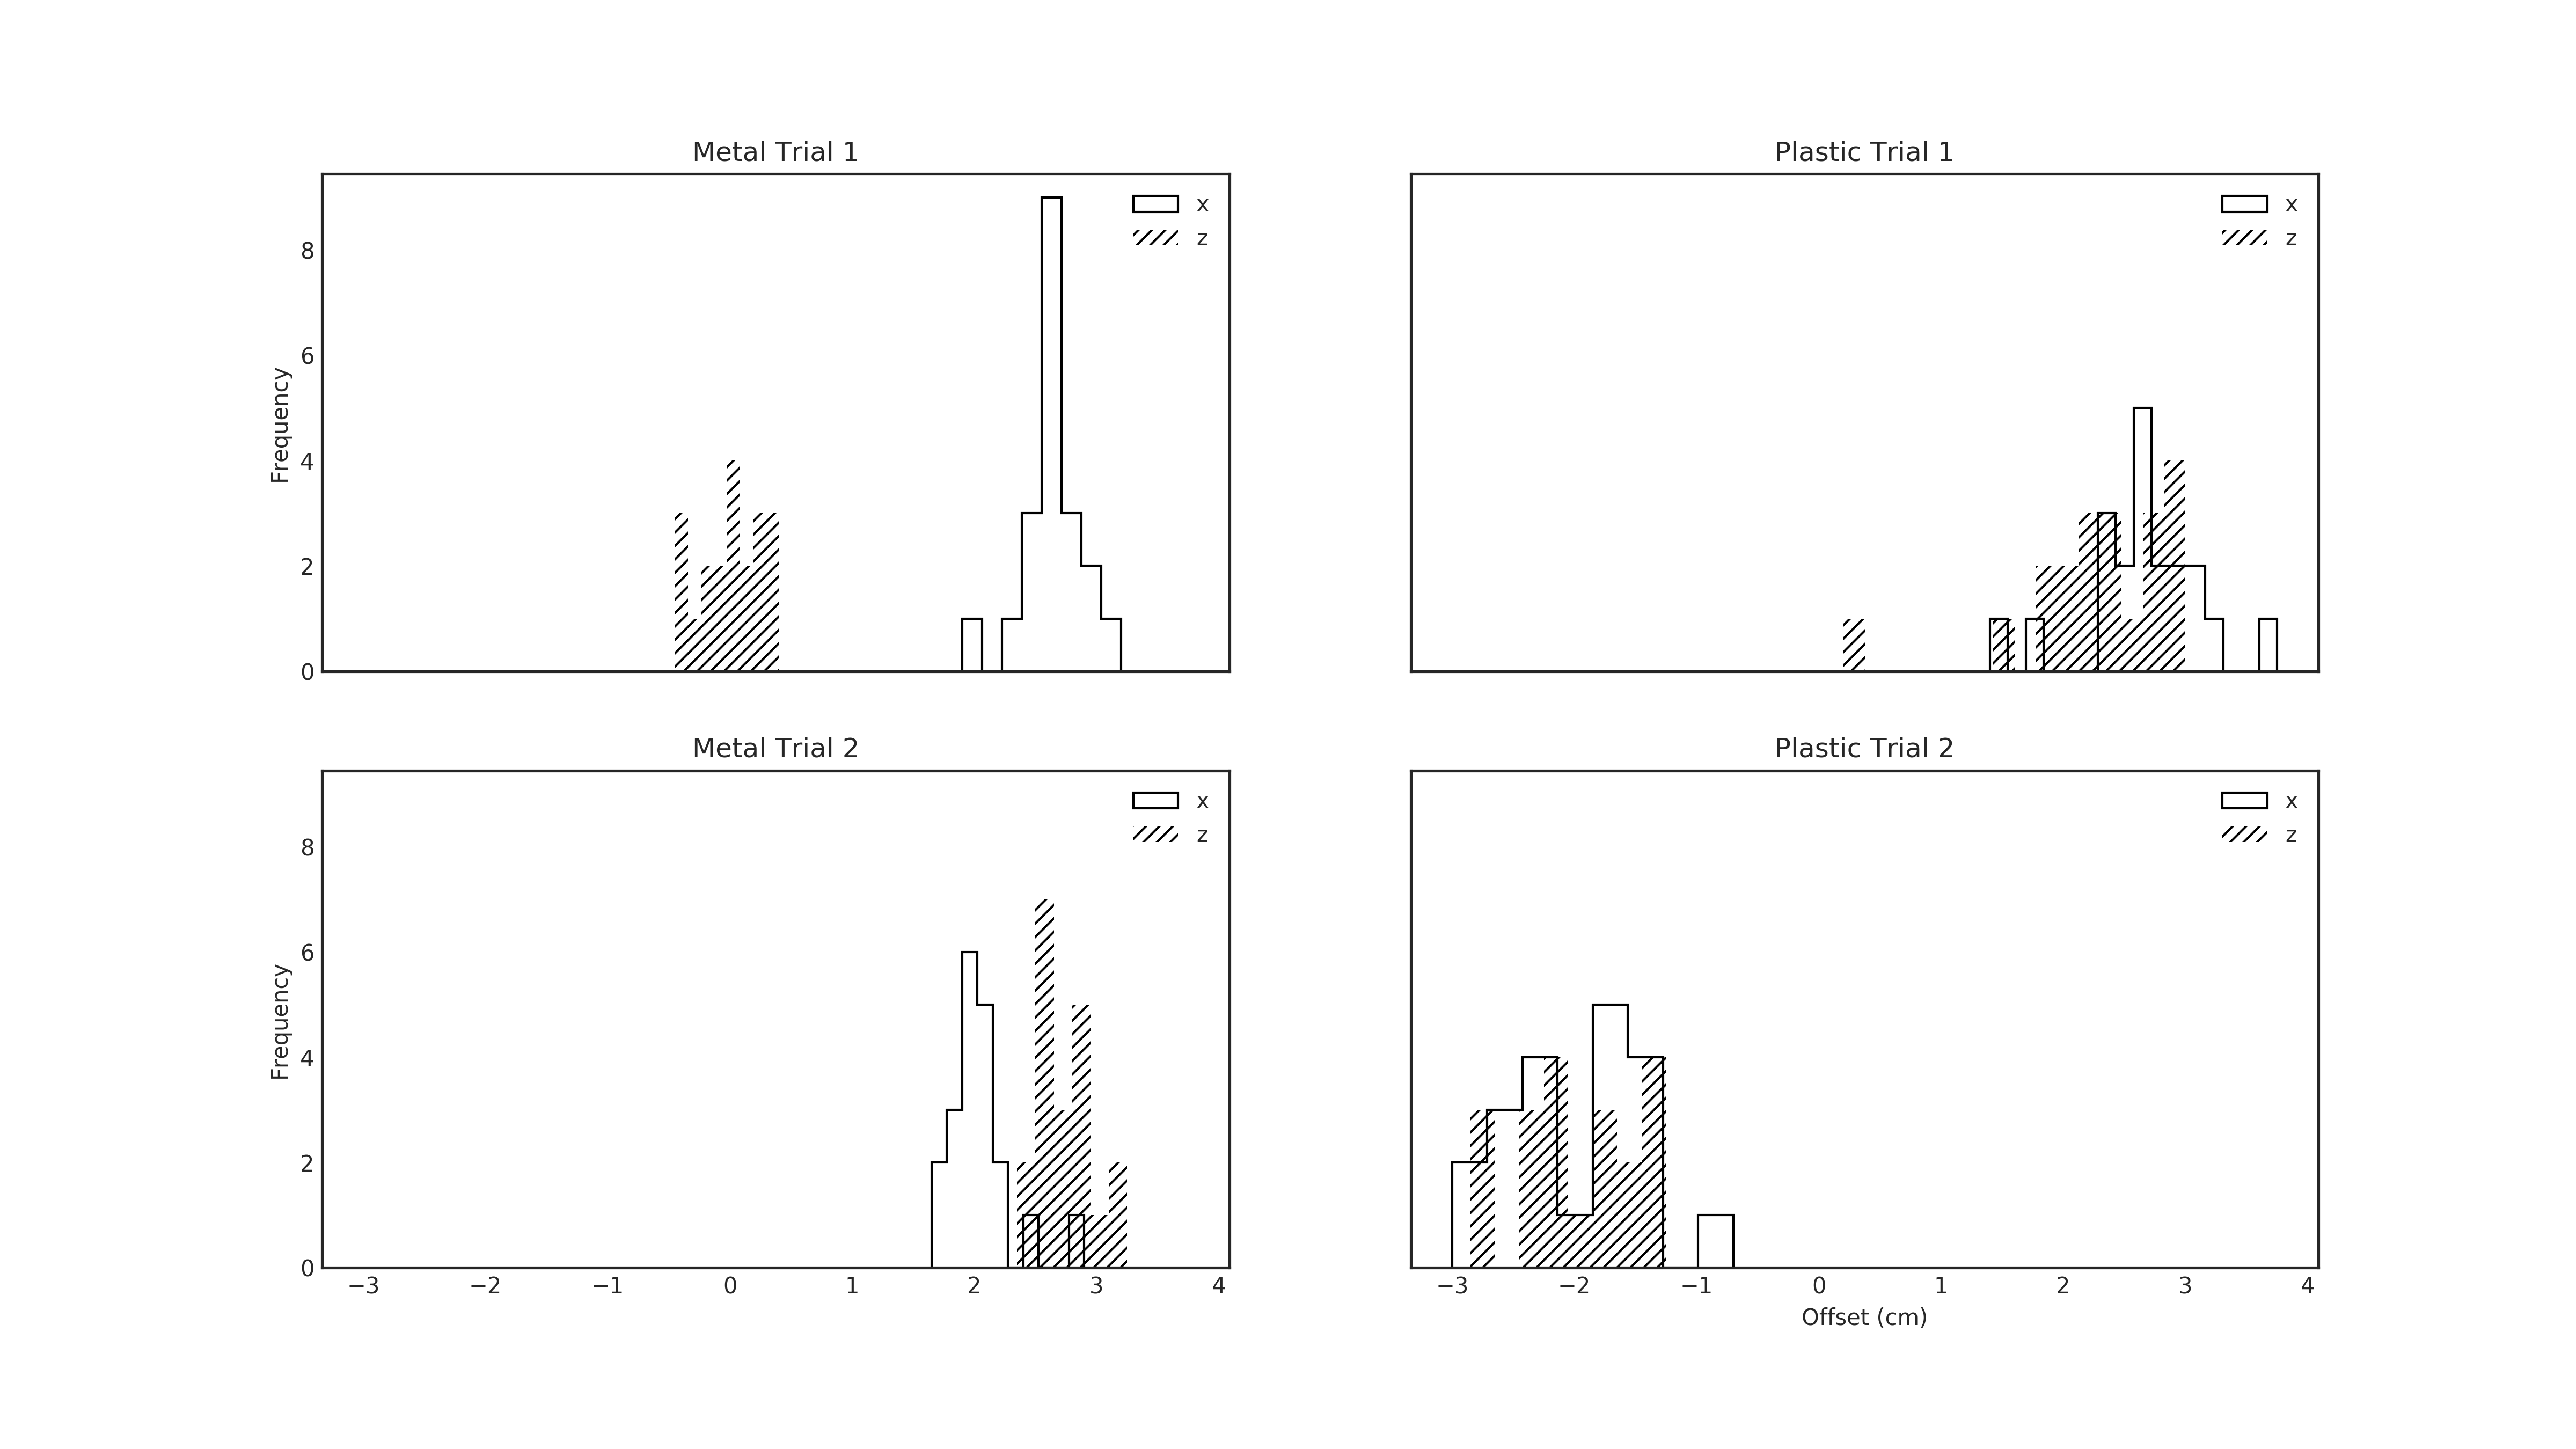
\includegraphics[width=1\textwidth]{hist_300.png} % Include the image placeholder.png
    \caption{Difference between actual and expected positions}
    \label{fig:hist}
\end{center}
\end{sidewaysfigure}

%----------------------------------------------------------------------------------------
%   Conclusions
%----------------------------------------------------------------------------------------
\clearpage
\section{Conclusions}

All the distributions are roughly bell-shaped, as seen in figure \ref{fig:hist}, but only the first trial of the metal sphere has a distribution centered around the expected value. In the remaining trials, the overall shift in the points is evident of systematic errors. Many factors could have caused this shift ---e.g., the presence of wind in the room toward one direction or an offset in the direction of the release ramp. 
\\\\
In each trial, the degree of spread in the x and z directions are similar. However, the trials for the metal sphere had significantly smaller spread than those of the plastic balls. This may be because metal balls have more mass, and thus their trajectories are less prone being affected by the random changes in the wind. Furthermore, the plastic is not a conductor, which means that it is able to hold a charge. The plastic's trajectory may be affected by electromagnetic forces. Altercations to reduce spread include performing the experiment in a vacuum, getting rid of static electricity, using denser spheres such as those made from lead. 
\\\\
If instead, a hollow plastic sphere was used for the experiment, its moment of inertia would increase. This would cause $v_{0}$ to decrease since a greater share of the gravitational potential energy is now converted to angular momentum. As a result, mean distance would decrease. 
\\\\
Our measurement of friction is relatively accurate. After measuring the work done by friction, we change the angle of release for the slide which may alter the amount of work done by friction. This change should be fairly minimal, since the change in angle is very small. Another small factor is that the ball is not completely round. Since we release the ball from a random orientation, the sides of the ball contacting the slide are different each time the ball is released.
\\\\
To estimate the force of friction, we need to find the length of the tube. This can be estimated by can splitting the length of the tube into two segments $l_{1}$ and $l_{2}$. The segment where the ball slides down, and the segment where the ball goes back up. The latter, we have already measured: $l_{2} = L$. For the former, from the diagram it can be estimated that it has a slope of $\ang{30}$. We can thus calculate the length as follows: 
\begin{equation}
l = l_{1} + l_{2} = \frac{h_{1} - h_{2}}{sin(\ang{30})}+ L
\end{equation}

We calculate length to be roughly $70 \si{cm}$. However, this estimate is not very accurate since all the curves in the ramp are ignored for simplification. Since we never measured the mass of the ball, we will use the mass of the metal ball and assume it to be $5 \si{g}$. Using equation \eqref{eq:1}, we find:

\begin{equation}
    \frac{Wf}{L} = 1.4 * 10^{-3} \si{N}
\end{equation}

We can compare the force of friction to the force of gravity of the ball:

\begin{equation}
F = mg = 9.8\frac{\si{m}}{\si{s}^{2}} * 5^{-3} \si{g} = 4.9 * 10^{-2} \si{N}
\end{equation}

Since these values are only a magnitude of 10 apart, the force of gravity is significant.
\\\\
I expect the estimate to increase in some areas while decreasing in other areas. The normal force between the ball and the tube determines the magnitude of the frictional force. We expect this force to be maximal at the bottom of the ramp where it curves since the ball is subject to the greatest acceleration here.

 %----------------------------------------------------------------------------------------
 %   BIBLIOGRAPHY
 %----------------------------------------------------------------------------------------

 \bibliographystyle{apalike}

 \bibliography{sample}

 %----------------------------------------------------------------------------------------
 \end{document}
